\chapter{Control Óptimo y Planificación}

\lecture{10}{2020-06-18}{Optimal Control and Planning}

\section{Introducción a RL basado en modelo}%
\label{sec:introducción_a_rl_basado_en_modelo}

Hasta ahora en el curso, se usaba objetivo:

\begin{figure}[htpb]
	\centering
	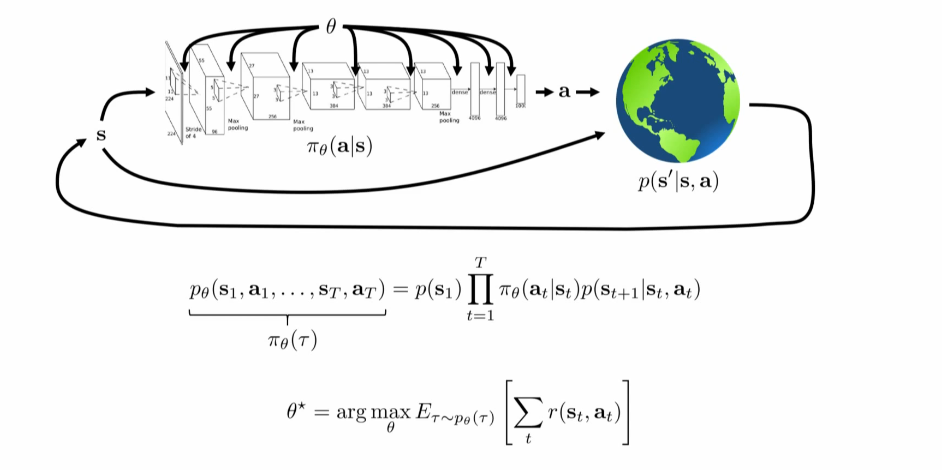
\includegraphics[width=0.8\linewidth]{figures/2020-06-18-112440_942x470_scrot.png}
\end{figure}

En el cual no se conocía $p(s_{t+1}|s_t,a_t)$. En RL basado en modelo se intenta aprender este
término con el bojetivo de tomar mejores acciones.

Normalmente, se conocen las dinámicas del entorno:
 \begin{enumerate}
     \item Videojuegos (Atari, Ajedrez, Go, ...)
     \item Sistemas fácilmente modelables (navegación de un coche)
     \item Entornos simulados (robots, videojuegos)
\end{enumerate}

También, nornalmente se pueden aprender las dinámicas:
\begin{enumerate}
    \item Identificación del sistema: ajustar los parámetros desconocidos de un modelo. Por
        ejemplo se usa para encontrar los parámetros desconocidos de un robot.
    \item Aprendizaje: ajustar un modelo de propósito general (como una red neuronal) a los
        datos que se tienen de las transiciones.
\end{enumerate}

\section{Si conocemos las dinámicas, ¿cómo se toman las decisiones?}%
\label{sec:si_conocemos_las_dinámicas_cómo_se_toman_las_decisiones_}

El objetivo es minimizar el coste:
\begin{align}
\operatorname { min } _ { a _ { 1 } , \ldots , a _ { T } } \sum _ { t = 1 } ^ { T } c ( s _ { t } , a _ { t } ) \text { s.t. } s _ { t } = f ( s _ { t - 1 } , a _ { t - 1 } )
\end{align}

En el caso determinista la dinámica del entorno está modelada por una función. Por lo que:
\begin{align}
a _ { 1 } , \ldots , a _ { T } = \operatorname { arg } \operatorname { max } _ { a _ { 1 } , \ldots , a _ { T } } \sum _ { t = 1 } ^ { T } r ( s _ { t } , a _ { t } ) \text { s.t. } s _ { t + 1 } = f ( s _ { t } , a _ { t } )
\end{align} 

En el caso estocástico de bucle abierto, las dinámicas están gobernadas por una distribución de
probabilidad. 
\begin{align}
p _ { \theta } ( s _ { 1 } , \ldots , s _ { T } | a _ { 1 } , \ldots , a _ { T } ) = p ( s _ { 1
} ) \prod ^ { T } p ( s _ { t + 1 } | s _ { t } , a _ { t } )\\
a _ { 1 } , \ldots , a _ { T } = \operatorname { arg } \operatorname { max } _ { a _ { 1 } ,
\ldots , a _ { T } } E \left[ \sum _ { t } r ( s _ { t } , a _ { t } ) | a _ { 1 } , \ldots , a _
{ T } \right]
\end{align}
El bucle abierto es muy ineficiente, ya que se tienen que coger todas las acciones para
terminar el episodio sólo con el estado inicial.

En el bucle cerrado, por otra parte, el agente recibe información del mundo después de haber
realizado una acción. En este caso, en vez de una secuencia de acciones lo que se tiene es una
política que se va siguiendo, como se ha visto hasta este tema.
\begin{align}
p ( s _ { 1 } , a _ { 1 } , \ldots , s _ { T } , a _ { T } ) = p ( s _ { 1 } ) \prod _ { t = 1 }
^ { T } \pi ( a _ { t } | s _ { t } ) p ( s _ { t + 1 } | s _ { t } , a _ { t } )\\
\pi = \operatorname { arg } \operatorname { max } _ { \pi } E _ { \tau \sim p ( \tau ) } \left[
    \sum _ { t } r ( s _ { t } , a _ { t } ) \right]
\end{align}

En este tema se explicarán varias formas de realizar la \textbf{planificación
en bucle abierto} por el momento.

\section{Métodos estocásticos de optimización}%
\label{sec:métodos_estocásticos_de_optimización}

Son optimizadores \textit{black-box} (da igual que sea planificación o control). Se abstrae
la planificación/control óptimo.
\begin{align}
a _ { 1 } , \ldots , a _ { T } = \operatorname { arg } \operatorname { max } _ { a _ { 1 } , \ldots , a _ { T } } J ( a _ { 1 } , \ldots , a _ { T } )
\end{align}
Realmente no importan las acciones tomadas, por lo que se escribe de la siguiente manera
(siendo $J$ el objetivo):
\begin{align}
A = \operatorname { arg } \operatorname { max } _ { A } J ( A )
\end{align}

No suele ser una buena idea optimizar esto usando gradientes, por lo que se suelen usar
optimizadores libres de derivadas (\textit{Derivative-free optimizers}) como MCTS o CEM. Esto es
porque suele ser difícil calcular derivadas de los entornos de simulación, por ejemplo en
MuJoCo es mucho más fácil crear episodios que calcular diferenciales.

El método más sencillo para hacer esto es simplemente 'suponer y probar':
\begin{enumerate}
    \item Escoger $A_1,\ldots,A_N$ de una distribución (por ejemplo uniforme).
    \item Escoger $A_i$ basándose en  $arg\max_iJ(A)$.
\end{enumerate}

Otra manera sencilla y popular de hacerlo mejor es el método de la entropía cruzada
(\textit{Cross-entropy method, CEM}). Consiste en hacer lo mismo varias veces, pero
actualizando la distribución de la cual se escogen las acciones. Funciona así, iterativamente:
\begin{enumerate}
    \item Se muestrea $ A_1, \ldots,A_N$ de $ p(A)$.
    \item Se evalúa $J(A_1,\ldots,J(A_N))$
    \item Se escogen los \textit{élites} $A_{i_1},\ldots,A_{i_M}$ con el mayor valor, donde
         $M<N$.
     \item Se ajusta $p(A)$ para los élites $A_{i_1},\ldots,A_{i_M}$. Se puede usar cualquier
         distribución para ajustar, pero normalmente una distribución normal multivariante
         funciona bien.
\end{enumerate}

(Nótese que $A_i$ es una trayectoria de $a_1,\ldots,a_K$).

CEM no es un optimizador muy bueno pero es muy sencillo y paralelizable. Como desventajas
tiene un límite de dimensionalidad muy fuerte y sólo hace planificación en bucle abierto.

Hay algoritmos similares pero un poco más complejos como CMA-ES, el cual se podría pensar que es
CEM con momento.

\section{Monte Carlo Tree Search}%
\label{sec:monte_carlo_tree_search}

Es otro método que gestiona el caso estocástico \textbf{discreto} de una forma más elegante.
También funciona en el caso continuo, pero es más complicado. Es muy popular para hacer
planificación en videojuegos.

La planificación crece exponencialmente con el número de pasos en el tiempo que se quiere
explorar.

\begin{figure}[H]
	\centering
	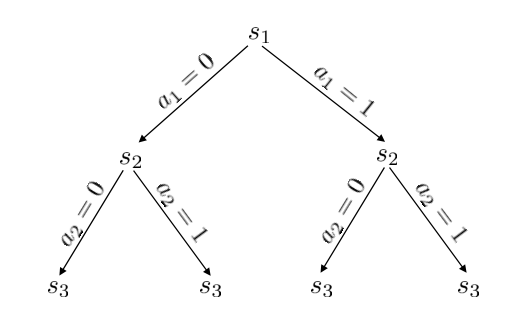
\includegraphics[width=0.4\linewidth]{figures/2020-06-18-122724_532x327_scrot.png}
\end{figure}

Las $s$ no se corresponden a estados sino a pasos en el tiempo. En vez de expandir el árbol
hasta el final del episodio, se puede expandir hasta un cierto punto y a partir de ahí tener
una estimación a partir de una política para ver si es un buen estado.

\begin{figure}[H]
	\centering
	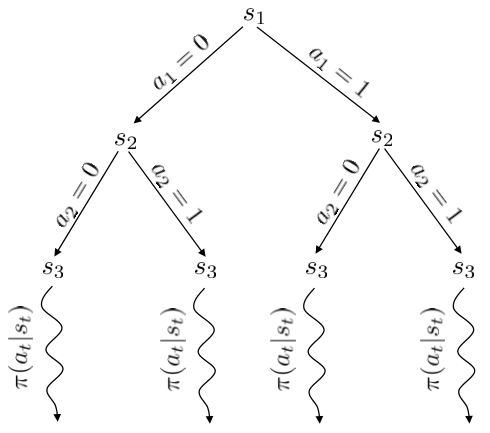
\includegraphics[width=0.4\linewidth]{figures/2020-06-18-122954_490x433_scrot.png}
	\caption{La política puede ser una política aleatoria por ejemplo.}
\end{figure}

La intuición es que a partir de 'desenrollar' los posibles estados inmediatos a los que
se puede llegar y después añadir una política 'estúpida' que recoja una aproximación al
valor de ese camino, se puede estimar cuál de las acciones es la más adecuada tomar.

Una de las mejoras más inmediatas a MCTS es entrenar una política en vez de usar una aleatoria.

Además, al no poder buscar por todos los caminos es interesante expandir los caminos que
inicialmente tengan más recompensa. Esto no garantiza que se encuentre un mejor camino al
final. También es posible preferir expandir nodos que no se visiten mucho, ya que quedan por
explorar y se podría encontrar en esos un camino mejor.

Un boceto general del algoritmo MTCS puede ser el siguiente (iterativamente):
\begin{enumerate}
    \item Encontrar una hoja $s_l$ usando un TreePolicy($s_1$). TreePolicy no es una política,
        sino una estrategia mediante la que se elige que hoja expandir.
    \item Evaluar la hoja usando DefaultPolicy($s_l$). DefaultPolicy sí que es una política y se
        evalúa 'jugando' hasta el final del juego.
    \item Se actualizan todos los valores del árbol entre $s_1$ y $s_l$.
\end{enumerate}
Al final, se elije la mejor acción desde $s_1$, repitiendo todo el proceso para el siguiente
estado.

En cada nodo del árbol se guarda el valor de todas las recompensas, contando las obtenidas por la
política 'tonta' ($Q$) y también se guarda el número de veces que se ha visitado ese nodo
($N$).

TreePolicy se puede formular de la siguiente forma:
\begin{itemize}
    \item Si $s_t$ no ha sido totalmente expandido, escoger esa nueva acción $a_t$.
    \item En caso contrario, escoger al hijo con la mayor puntuación.
\end{itemize}
La puntuación es algo que se puede elegir arbitrariamente, y pretende balancear la
relación de puntuación $Q$ y el número de veces que se ha visitado un nodo $N$ (para valores
menores de $N$, que sea más probable visitarlo). Una relación que se suele usar es:
\begin{align}
\operatorname { Score } ( s _ { t } ) = \frac { Q ( s _ { t } ) } { N ( s _ { t } ) } + 2 C \sqrt { \frac { 2 \operatorname { ln } N ( s _ { t - 1 } ) } { N ( s _ { t } ) } }
\end{align}
Donde $C$ es un hiperparámetro.

\begin{figure}[H]
	\centering
	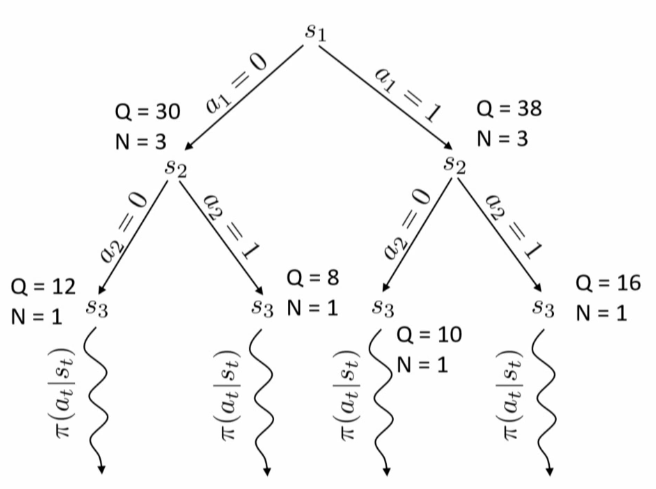
\includegraphics[width=0.5\linewidth]{figures/2020-06-18-154825_656x489_scrot.png}
	\caption{Ejemplo de un árbol expandido.}
\end{figure}

\section{Optimización de trayectorias}%
\label{sec:optimización_de_trayectorias}

Estos métodos se usan en los casos en los que se puedan obtener derivadas del entorno (por
ejemplo modelos dinámicos de un robot). En control óptimo, los estados se representan como
$x_t$ y las acciones (control) como  $u_t$. El objetivo en vez de maximizar una recompensa es el
de minimizar un coste:
\begin{align}
\operatorname { min } _ { u _ { 1 } , \ldots , u _ { T } } \sum _ { t = 1 } ^ { T } c ( x _ { t } , u _ { t } ) \text { s.t. } x _ { t } = f ( x _ { t - 1 } , u _ { t - 1 } )
\end{align}
Por ahora, se supone que los problemas son deterministas. La ecuación de arriba representa un
problema de optimización con restricciones, pero se pueden quitar las restricciones
expresándolo recursivamente como:
\begin{align}
    \label{eq:shootingmethod}
\operatorname { min } _ { u _ { 1 } , \ldots , u _ { T } } c ( x _ { 1 } , u _ { 1 } ) + c ( f ( x _ { 1 } , u _ { 1 } ) , u _ { 2 } ) + \cdots + c ( f ( f ( \ldots ) \ldots ) , u _ { T } )
\end{align}
Se se tiene una desigualdad como restricción, es muy fácil de sustituir.


Para optimizar esto usando técnicas de descenso por gradiente se necesita $\frac { d f } { d x _
{ t } } , \frac { d f } { d u _ { t } } , \frac { d c } { d x _ { t } } , \frac { d c } { d u _ {
t } }$. En muchos casos de control óptimo, no es una buena idea intentar optimizarlo mediante
un optimizador de primer orden y se suelen usar optimizadores de segundo orden.

La expresión \ref{eq:shootingmethod} se llama \textit{Shooting Method}, se llama así porque se
está optimizando sobre acciones y los estados son consecuencia de esas acciones. Estos
sistemas tienen la propiedad de que cambios pequeños en las acciones del principio llevan a
cambios grandes en los estados más avanzados. Numéricamente esto son malas noticias, ya que
significa que podemos ser extremadamente sensibles a ciertos parámetros y totalmente
insensibles a otros.

Como alternativa existen los llamados \textit{Collocation method}, donde se están optimizando los
estados en vez de las acciones, imponiendo una restricción:
\begin{align}
\operatorname { min } _ { u _ { 1 } , \ldots , u _ { T } , x _ { 1 } , \ldots , x _ { T } } \sum _ { t = 1 } ^ { T } c ( x _ { t } , u _ { t } ) \text { s.t. } x _ { t } = f ( x _ { t - 1 } , u _ { t - 1 } )
\end{align}
Estos métodos se suelen resolver con programación cuadrática.

En este tema se explicarán los \textit{Shooting methods} donde en vez de usar descenso por
gradiente se usa LQR, que es un algoritmo de optimización de segundo orden parecido al método
de Newton pero sin la necesidad de calcular la matriz hessiana. 

Para derivar el algoritmo, se va a hacer con un problema mucho más sencillo, llamado
\textit{Linear Quadratic Regulator}. Es un problema de control donde se intenta minimizar el
coste como antes (expresión \ref{eq:shootingmethod}) pero $f(x_t,u_t)$ tiene una estructura especial (se asume que es lineal).
 \begin{align}
     \label{eq:linear}
f ( x _ { t } , u _ { t } ) = F _ { t } \left[ \begin{array} { l } { x _ { t } } \\ { u _ { t } } \end{array} \right] + f _ { t }
\end{align}
En general puede ser que se tenga una $F_t$ y  $f_t$ distintas en cada paso.

También se asume que el coste es cuadrático:
\begin{align}
    \label{eq:quadratic}
c ( x _ { t } , u _ { t } ) = \frac { 1 } { 2 } \left[ \begin{array} { c } { x _ { t } } \\ { u _ { t } } \end{array} \right] ^ { T } C _ { t } \left[ \begin{array} { c } { x _ { t } } \\ { u _ { t } } \end{array} \right] + \left[ \begin{array} { c } { x _ { t } } \\ { u _ { t } } \end{array} \right] ^ { T } c _ { t }
\end{align}
También se puede expresar con una constante sumada pero esto no cambia las acciones tomadas por
lo que no hace falta tenerlo en cuenta.

Las expresiones \ref{eq:linear} y \ref{eq:quadratic} van respectivamente en
\ref{eq:shootingmethod}.

Para empezar, se va a resolver para $u_T$, ya que al estar al final, no afecta a ningún
estado futuro porque no hay. El único término que depende de $u_T$ es
$c(f(f(\ldots)\ldots),u_T)$, donde  $x_T=f(f(\ldots)\ldots)$ y es desconocido.

El coste para este término es:
 \begin{align}
Q ( x _ { T } , u _ { T } ) = \text { const } + \frac { 1 } { 2 } \left[ \begin{array} { c } { x _ { T } } \\ { u _ { T } } \end{array} \right] ^ { T } C _ { T } \left[ \begin{array} { l } { x _ { T } } \\ { u _ { T } } \end{array} \right] + \left[ \begin{array} { l } { x _ { T } } \\ { u _ { T } } \end{array} \right] ^ { T } c _ { T }
\end{align}
El valor de $u_T$ que minimiza esta cantidad en términos de $x_T$. Como es una función
cuadrática, es convexa y su único mínimo es el global. Por lo que:
\begin{align}
    \nabla _ { u _ { T } } Q ( x _ { T } , u _ { T } ) &= C _ { u _ { T } , x _ { T } } x _ { T } + C
_ { u _ { T } , u _ { T } } u _ { T } + c _ { u _ { T } } ^ { T } = 0\\
    u _ { T } &= - C _ { u _ { T } , u _ { T } } ^ { - 1 } ( C _ { u _ { T } , x _ { T } } x _ { T } + c _ { u _ { T } } )
    \label{eq:ut}
\end{align}

Donde:
\begin{align}
    C _ { T } &= \left[ \begin{array} { l l } { C _ { x _ { T } , x _ { T } } } & { C _ { x _ { T
    } , u _ { T } } } \\ { C _ { u _ { T } , x _ { T } } } & { C _ { u _ { T } , u _ { T } } }
                \end{array} \right]\\
                c _ { T } &= \left[ \begin{array} { l } { c _ { x _ { T } } } \\ { c _ { u _ { T } } } \end{array} \right]
\end{align}

Para simplificar, se expresa \ref{eq:ut} como $u_T=K_Tx_T+k_T$, donde
$K_T=-C^{-1}_{u_T,u_T}C_{u_T,x_T}$ y  $k_T=-C^{-1}_{u_T,u_T}c_{u_T}$. Se ha expresado la mejor
acción final como una función lineal del estado final.

Ahora se procede de forma recursiva hacia atrás en el tiempo. Como  $u_T$ está completamente
determinado por $x_T$, se puede eliminar $u_T$ mediante sustitución.
\begin{align}
    \label{eq:Vshoot}
V ( x _ { T } ) = \operatorname { const } + \frac { 1 } { 2 } \left[ \begin{array} { c } { x _ { T } } \\ { K _ { T } x _ { T } + k _ { T } } \end{array} \right] ^ { T } C _ { T } \left[ \begin{array} { c } { x _ { T } } \\ { K _ { T } x _ { T } + k _ { T } } \end{array} \right] + \left[ \begin{array} { c } { x _ { T } } \\ { K _ { T } x _ { T } + k _ { T } } \end{array} \right] ^ { T } c _ { T }
\end{align}
Si se expande, se obtiene:
\begin{align}
\left. \begin{array}{l}{ V ( x _ { T } ) = \frac { 1 } { 2 } x _ { T } ^ { T } C _ { x _ { T } , x _ { T } } x _ { T } + \frac { 1 } { 2 } x _ { T } ^ { T } C _ { x _ { T } , u _ { T } } K _ { T } x _ { T } + \frac { 1 } { 2 } x _ { T } ^ { T } K _ { T } ^ { T } C _ { u _ { T } , x _ { T } } x _ { T } + \frac { 1 } { 2 } x _ { T } ^ { T } K _ { T } ^ { T } C _ { u _ { T } , u _ { T } } K _ { T } x _ { T } + }\\{ x _ { T } ^ { T } K _ { T } ^ { T } C _ { u _ { T } , u _ { T } } k _ { T } + \frac { 1 } { 2 } x _ { T } ^ { T } C _ { x _ { T } , u _ { T } } k _ { T } + x _ { T } ^ { T } c _ { x _ { T } } + x _ { T } ^ { T } K _ { T } ^ { T } c _ { u _ { T } } + \text { const } }\end{array} \right.
\end{align}
Para simplificar la notación, esto se expresa como:
\begin{align}
V ( x _ { T } ) = const + \frac { 1 } { 2 } x _ { T } ^ { T } V _ { T } x _ { T } + x _ { T } ^ { T } v _ { T }
\end{align}
Donde:
\begin{align}
\left. \begin{array} { l } { V _ { T } = C _ { x _ { T } , x _ { T } } + C _ { x _ { T } , u _ { T } } K _ { T } + K _ { T } ^ { T } C _ { u _ { T } , x _ { T } } + K _ { T } ^ { T } C _ { u _ { T } , u _ { T } } K _ { T } } \\ { v _ { T } = c _ { x _ { T } } + C _ { x _ { T } , u _ { T } } k _ { T } + K _ { T } ^ { T } C _ { u _ { T } } + K _ { T } ^ { T } C _ { u _ { T } , u _ { T } } k _ { T } } \end{array} \right.
\end{align}

Ahora se resuelve $u_{T-1}$ en términos de $x_{T-1}$. Pero se tiene que tener en cuenta que
$x_T$ también está afectado por $u_{T-1}$ de la siguiente manera:
\begin{align}
    f ( x _ { T - 1 } , u _ { T - 1 } ) &= x _ { T } = F _ { T - 1 } \left[ \begin{array} { c } { x _
{ T - 1 } } \\ { u _ { T - 1 } } \end{array} \right] + f _ { T - 1 }\\
Q(x_{T-1},u_{T-1}) &= \text { const } + \frac { 1 } { 2 } \left[ \begin{array} { c } { x _ { T - 1 } } \\ { u _ { T - 1 } } \end{array} \right] ^ { T } C _ { T - 1 } \left[ \begin{array} { c } { x _ { T - 1 } } \\ { u _ { T - 1 } } \end{array} \right] + \left[ \begin{array} { c } { x _ { T - 1 } } \\ { u _ { T - 1 } } \end{array} \right] ^ { T } c _ { T - 1 } + V ( f ( x _ { T - 1 } , u _ { T - 1 } ) )
\end{align}
Donde el último término se corresponde con \ref{eq:Vshoot}. Si se expande, queda:
\begin{align}
V ( x _ { T } ) = \operatorname { const } + \frac { 1 } { 2 } \left[ \begin{array} { c } { x _ { T - 1 } } \\ { u _ { T - 1 } } \end{array} \right] ^ { T } F _ { T - 1 } ^ { T } V _ { T } F _ { T - 1 } \left[ \begin{array} { c } { x _ { T - 1 } } \\ { u _ { T - 1 } } \end{array} \right] + \left[ \begin{array} { c } { x _ { T - 1 } } \\ { u _ { T - 1 } } \end{array} \right] ^ { T } F _ { T - 1 } ^ { T } V _ { T } f _ { T - 1 } + \left[ \begin{array} { c } { x _ { T - 1 } } \\ { u _ { T - 1 } } \end{array} \right] ^ { T } F _ { T - 1 } ^ { T } v _ { T }
\end{align}
Que si se simplifica, queda como:
\begin{align}
Q ( x _ { T - 1 } , u _ { T - 1 } ) = \operatorname { const } + \frac { 1 } { 2 } \left[ \begin{array} { c } { x _ { T - 1 } } \\ { u _ { T - 1 } } \end{array} \right] ^ { T } Q _ { T - 1 } \left[ \begin{array} { c } { x _ { T - 1 } } \\ { u _ { T - 1 } } \end{array} \right] + \left[ \begin{array} { c } { x _ { T - 1 } } \\ { u _ { T - 1 } } \end{array} \right] ^ { T } q _ { T - 1 }
\end{align}
Que se puede ver perfectamente que vuelve a tener un término cuadrático y otro término lineal.
Para hacer esta simplificación, se tiene en cuenta que:
\begin{align}
\left. \begin{array} { l } { Q _ { T - 1 } = C _ { T - 1 } + F _ { T - 1 } ^ { T } V _ { T } F _ { T - 1 } } \\ { q _ { T - 1 } = c _ { T - 1 } + F _ { T - 1 } ^ { T } V _ { T } f _ { T - 1 } + F _ { T - 1 } ^ { T } v _ { T } } \end{array} \right.
\end{align}

Como en el primer paso, se vuelve a calcular la derivada de esta expresión y se iguala a 0 para
obtener el mínimo. Al hacer esto queda de solución:
\begin{align}
u _ { T - 1 } = K _ { T - 1 } x _ { T - 1 } + k _ { T - 1 }
\end{align}
Donde:
\begin{align}
K _ { T - 1 } = - Q _ { u _ { T - 1 } , u _ { T - 1 } } ^ { - 1 } Q _ { u _ { T - 1 } , x _ { T - 1 } } \quad k _ { T - 1 } = - Q _ { u _ { T - 1 } , u _ { T - 1 } } ^ { - 1 } q _ { u _ { T } }
\end{align}

Esto se repite hasta llegar al paso inicial.

Por lo que el algoritmo queda como:
\begin{algorithm}
    \caption{LQR}
    \For{t=T hasta 1}{
        $ \left. \begin{array} { l } { Q _ { t } = C _ { t } + F _ { t } ^ { T } V _ { t + 1 } F _ { t } } \\ { q _ { t } = c _ { t } + F _ { t } ^ { T } V _ { t + 1 } f _ { t } + F _ { t } ^ { T } v _ { t + 1 } } \\ { Q ( x _ { t } , u _ { t } ) = \operatorname { const } + \frac { 1 } { 2 } \left[ \begin{array} { c } { x _ { t } } \\ { u _ { t } } \end{array} \right] ^ { T } Q _ { t } \left[ \begin{array} { c } { x _ { t } } \\ { u _ { t } } \end{array} \right] + \left[ \begin{array} { c } { x _ { t } } \\ { u _ { t } } \end{array} \right] ^ { T } q _ { t } } \\ { u _ { t } \leftarrow \operatorname { arg } \operatorname { min } _ { u _ { t } } Q ( x _ { t } , u _ { t } ) = K _ { t } x _ { t } + k _ { t } } \\ { K _ { t } = - Q _ { u _ { t } , u _ { t } } ^ { - 1 } Q _ { u _ { t } , x _ { t } } } \\ { k _ { t } = - Q _ { u _ { t } , u _ { t } } ^ { - 1 } q _ { u _ { t } } } \\ { V _ { t } = Q _ { x _ { t } , x _ { t } } + Q _ { x _ { t } , u _ { t } } K _ { t } + K _ { t } ^ { T } Q _ { u _ { t } , x _ { t } } + K _ { t } ^ { T } Q _ { u _ { t } , u _ { t } } K _ { t } } \\ { v _ { t } = q _ { x _ { t } } + Q _ { x _ { t } , u _ { t } } k _ { t } + K _ { t } ^ { T } Q _ { u _ { t } } + K _ { t } ^ { T } Q _ { u _ { t } , u _ { t } } k _ { t } } \\ { V ( x _ { t } ) = \operatorname { const } + \frac { 1 } { 2 } x _ { t } ^ { T } V _ { t } x _ { t } + x _ { t } ^ { T } v _ { t } } \end{array} \right.  $
    }
\end{algorithm}

Cuando se finaliza, se llega al estado inicial $x_1$ el cual es conocido. Ahora lo que se hace
es avanzar recursivamente hacia adelante para calcular todas las $u_t$.

\begin{algorithm}
    \caption{LQR: recursión hacia adelante}
    \For{t=1 hasta T}{
        $ \left. \begin{array} { l } { u _ { t } = K _ { t } x _ { t } + k _ { t } } \\ { x _ { t
        + 1 } = f ( x _ { t } , u _ { t } ) } \end{array} \right.$
    }
\end{algorithm}

El algoritmo descrito es de bucle abierto, pero se puede modificar para que se vuelva de bucle
cerrado.

Este algoritmo es muy eficiente ya que las inversiones de las matrices que hay que hacer son de
dimensionalidades bajas (porque es la dimensionalidad del espacio de acciones).

En este algoritmo, $Q_t$ y $v_t$ son literalmente sus funciones valor correspondientes en
la formulación de RL (salvo que ahora el $v$ en vez de ser el máximo de sus $Q$ es el mínimo,
porque se está minimizando el coste).

En el caso de que se tengan \textbf{dinámicas estocásticas} y sean gaussianas
(mientras la covarianza sea constante), la
solución es exactamente la misma.

Este algoritmo sirve para resolver sistemas lineales. Para \textbf{sistemas no lineales} se
puede extender el algoritmo a otro llamado LQR Iterativo o Programación Dinámica
Diferencial (DDP en inglés).

Su funcionamiento se basa en la aproximación de los sistemas no lineales mediante series de
Taylor en el entorno local. Concretamente, una aproximación lineal de la dinámica y una
aproximación cuadrática del coste.

\begin{align}
    f ( x _ { t } , u _ { t } ) &\approx f ( \hat { x } _ { t } , \hat { u } _ { t } ) + \nabla _
    { x _ { t } , u _ { t } } f ( \hat { x } _ { t } , \hat { u } _ { t } ) \left[ \begin{array}
    { c } { x _ { t } - \hat { x } _ { t } } \\ { u _ { t } - \hat { u } _ { t } } \end{array}
\right]\\
c(x_t,u_t)&\approx c ( \hat { x } _ { t } , \hat { u } _ { t } ) + \nabla _ { x _ { t } , u _ { t } } c ( \hat { x } _ { t } , \hat { u } _ { t } ) \left[ \begin{array} { c } { x _ { t } - \hat { x } _ { t } } \\ { u _ { t } - \hat { u } _ { t } } \end{array} \right] + \frac { 1 } { 2 } \left[ \begin{array} { c } { x _ { t } - \hat { x } _ { t } } \\ { u _ { t } - \hat { u } _ { t } } \end{array} \right] ^ { T } \nabla _ { x _ { t } , u _ { t } } ^ { 2 } c ( \hat { x } _ { t } , \hat { u } _ { t } ) \left[ \begin{array} { c } { x _ { t } - \hat { x } _ { t } } \\ { u _ { t } - \hat { u } _ { t } } \end{array} \right]
\end{align}
Se define $\delta x_t=x_t-\hat{x}_t$ y $\delta u=u_t-\hat{u}_t$ ($\hat{x}$ y $\hat{u}$ son las
trayectorias que se tenían en la iteración anterior).
\begin{align}
\left. \begin{array}{l}{ \overline { f } ( \delta x _ { t } , \delta u _ { t } ) = F _ { t }
    \left[ \begin{array} { c } { \delta x _ { t } } \\ { \delta u _ { t } } \end{array} \right]
    }\\{F_t = \nabla _ { x _ { t } , u _ { t } } f ( \hat { x } _ { t } , \hat { u } _ { t } )
    }\end{array} \right.\\
\left. \begin{array}{l}{ \overline { c } ( \delta x _ { t } , \delta u _ { t } ) = \frac { 1 } {
    2 } \left[ \begin{array} { c } { \delta x _ { t } } \\ { \delta u _ { t } } \end{array}
    \right] ^ { T } C _ { t } \left[ \begin{array} { c } { \delta x _ { t } } \\ { \delta u _ { t
    } } \end{array} \right] + \left[ \begin{array} { l } { \delta x _ { t } } \\ { \delta u _ { t
    } } \end{array} \right] ^ { T } c _ { t } }\\{ C_t=\nabla _ { x _ { t } , u _ { t } } ^ { 2 }
    c ( \hat { x } _ { t } , \hat { u } _ { t } )\quad c_t= \nabla _ { x _ { t } , u _ { t } } c ( \hat { x } _ { t } , \hat { u } _ { t } ) }\end{array} \right.
\end{align}

Con esto, se ejecuta el algoritmo LQR que se tenía antes. 

\begin{algorithm}
    \caption{LQR Iterativo}
    \While{no haya convergido}{
$
\left. \begin{array} { l } { F _ { t } = \nabla _ { x _ { t } , u _ { t } } f ( \hat { x } _ { t } , \hat { u } _ { t } ) } \\ { c _ { t } = \nabla _ { x _ { t } , u _ { t } } c ( \hat { x } _ { t } , \hat { u } _ { t } ) } \\ { C _ { t } = \nabla _ { x _ { t } , u _ { t } } ^ { 2 } c ( \hat { x } _ { t } , \hat { u } _ { t } ) } \end{array} \right.
$\\
    Ejecutar el paso hacia atrás de LQR en el estado $\delta x_t$ y acción  $\delta u_t$.\\
    Ejecutar el paso hacia adelante con la dinámica no lineal real y
    $u_t=K_t(x_t-\hat{x}_t)+k_t+\hat{u}_t$\\
    Actualizar $\hat{x}_t$ u $\hat{u}_t$ basándose en los estados y las acciones del paso
    hacia adelante.
    }
\end{algorithm}

Este algoritmo se parece bastante al método de Newton. Básicamente es el método de Newton
aplicado a la optimización de trayectorias. La única diferencia es que el método de Newton
usaría una aproximación de segundo orden para aproximar el estado.

Publicación relacionada: \textit{Synthesis and Stabilization of Complex Behaviors through
Online Trajectory Optimization}. Proporciona una guía práctica para implementar LQR
iterativo.
